\documentclass[PWPL]{article}
\usepackage{PWPL}
\usepackage{tipa}
\usepackage{enumerate}
\usepackage{graphicx}
\usepackage{multirow}
\usepackage{amsmath}
\usepackage{caption}
\usepackage{subfigure}
\title{The Social Perception of a Sound Change}
\author{Daniel Lawrence}
\begin{document}
\maketitle
%\abstract{A core claim of sociolinguistic theory is that language variation functions as a social-semiotic resource, providing an explanation for patterns of group-level convergence and divergence with regard to ongoing linguistic change. What is lacking from existing work is a framework for formulating testable hypotheses regarding the relationship between listeners’ social perceptions of innovations and their productive behavior with regard to those innovations. With a view to addressing this problem, this paper presents an account of the fronting and diphthongization of the tense back vowels \textipa{/u/} and \textipa{/o/} in York, Northern England. After presenting evidence of ongoing change in these vowels, the paper evaluates a recent account of the role of social indexicality in constraining the changes through a novel experimental paradigm. The findings contradict previous accounts of change in this community -- for example, despite its rapid and uniform incrementation and apparent lack of class-stratification in production, \textipa{/u/}-fronting emerges as a robust cue to socioeconomic status in perception. While the absence of fronted \textipa{/o/} monophthongs in the speech of younger speakers has previously been interpreted as evidence of their stigmatization, there is no support for this in the perception data. Intriguingly, there is evidence of structured variability in listeners’ social-perceptual responses -- the social groups who lead the changes in production appear to be more sensitive to their social-indexical significance in perception.}

\section{Introduction}

A core finding of sociolinguistic research is that phonological changes may attach to social distinctions as they propagate through a speech community. The social evaluations attached to innovations are often used as an explanation for changes in the trajectories of parallel vowel shifts (e.g. Labov et al. 2014), or to explain differences in the rates of adoption of innovations across social groups (e.g. Hall-Lew, 2009). While much work has framed these evaluations by referring to the degree of \textit{prestige} or \textit{stigma} attached to competing variants, recent studies have attempted to develop a more sophisticated understanding of the types of social meaning which may attach to variation. In particular, the notion of the \textit{persona} has risen to prominence -- it is argued that speaker-listeners' social perceptions of linguistic variation tend to be structured around locally-relevant stereotypical figures such as the `valley girl' or `burnout' (Eckert, 2008; Moore \& Podesva, 2009; D'onofrio, 2015). Applying this perspective to sound change, it has been argued that innovations which come about due to global processes of change (such as chain-shifting principles) may become attached to locally-meaningful stereotypes in certain speech communities, constraining the propagation of sound changes through social and geographic space. 

While this approach provides an intuitive account of how global processes might interact with local social-semiotic systems in influencing the outcome of a sound change, it raises an important methodological issue: how can the social meanings proposed for a given change can be verified, and how can their role in constraining that change be diagnosed? The present study explores this problem through an analysis of \textipa{/u/} and \textipa{/o/} fronting in York, Northern England. After providing evidence for ongoing change in \textipa{/u/} and \textipa{/o/}, a recent account of the role of social meaning in constraining these changes (Haddican et al. 2013) will be reviewed. This account will be evaluated in light of results from a controlled social perception experiment, which enable the testing of quantitative predictions regarding the perceptual mapping of phonetic cues to social categories across listener groups.


%\subsection{Sampling}

%Data are taken from a corpus of recordings collected from a convenience sample of 52 York residents born between 1935 and 2000. All participants were born and raised in York, and had at least one parent from York.Table 1 provides the basic demographic information of the sample, including participants' gender and year of birth (collected from a post-interview questionnaire), and their grouping according to a \textit{mobility index}. This index was one of three factors derived from informants' responses to the interview questions (see section x.x).

%\vspace*{6pt}
%\begin{table}[ht]
%\small
%\centering
%\begin{tabular}{l|l|l|l|l}
%Mobility index&\multicolumn{2}{l|}{Upper}&\multicolumn{2}{l}{Lower}\\
%\hline
%Gender& Female& Male & Female & Male\\
%\hline
%1935-1960 & 6&5&2&2\\
% 1961-1980& 2 &4&4&0\\
%1981-2000&  8&11&3&5\\

%\end{tabular}
%\caption{Characteristics of the speaker sample}
%\end{table}
%\vspace*{6pt}

%\subsection{Social coding}

%In addition to collecting each speaker's year of birth and gender, three social indices were created based on a set of questions asked during the sociolinguistic interview. Three underlying dimensions were derived from an exploratory factor analysis of these responses -- a general SES index, a local identity index, and a mobility index; for brevity, the specific details of this factor analysis will be left for a future version of this work. The general SES index groups together a measure of the speaker's level of education and employment status. The local identity index measures the degree to which each individual identifies as someone from York, and the extent to which they are invested in the local community. The mobility index groups together a set of characteristics related to geographical and social mobility, e.g. whether or not the speaker travels regularly within the UK; whether or not they have worked and studied in York for an extended period, and whether or not they plan to stay in York permanently.

%\subsection{Production data}

%The data include a) a 100-item wordlist, including 15 tokens of each vowel in a range of phonetic environments plus fillers; b) a map task (Anderson et al., 1991) using a selection of words from the word list and c) a sociolinguistic interview, including a range of questions relevant to the speakers' social background and identity with regard to York and the north of England. 

%Vowels were segmented from the first to the last glottal pulse visible in the spectrogram, and measurements of F1, F2 and F3 were taken at 20 equidistant points along the vowel trajectory. The present analysis will focus on F2 trajectories, which provide a relatively reliable reflection of the degree of fronting and diphthongization for these vowels. Measurements were normalized using the centroid method of Watt \& Fabricius (2002), using the mean midpoint values of each speakers' \textipa{/A/} and \textipa{/i/} productions as reference values. The formant values provided in the present analyses are of the form $F^n/S (F^n)$, i.e. the ratio of the measured frequency in Hz to the centroid frequency of that formant for the speaker being analyzed.


\section{\textipa{/u/} and \textipa{/o/} fronting in York, Northern England}
The data for the present study are taken from a corpus of sociolinguistic interviews collected from a convenience sample of 52 York residents born between 1935 and 2000. 40 tokens per vowel per speaker were extracted a range of phonetic environments, and F1 and F2 measurements were taken at 20 equidistant points along the vowel trajectory. These values were normalized using the Watt \& Fabricius (2002) method. Figures 1(a) and 1(b) plot each speaker's mean midpoint F2 for each vowel as function of their year of birth. Both vowels show evidence of fronting, but the fronting of \textipa{/o/} appears to be less regular than the fronting of \textipa{/u/}, evidenced by the fact that speaker means are less tightly clustered around the regression line in 1(b) than 1(a). The slope of change in \textipa{/u/} is also steeper than that for \textipa{/o/}, indicating more rapid change. These data suggest that \textipa{/u/} may be fronting in a more rapid and uniform manner than \textipa{/o/}.
\begin{figure}[!ht]
\centering
\caption{Variation and change in \textipa{/o/} and \textipa{/u/}}
\subfigure[]{
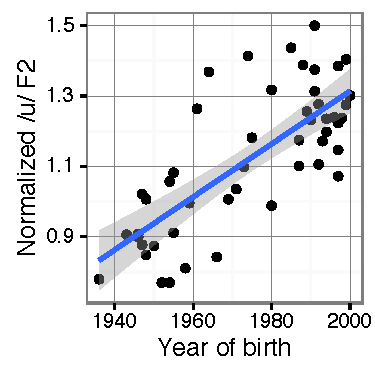
\includegraphics[scale=0.7]{uw_yob_small.pdf}}
\subfigure[]{
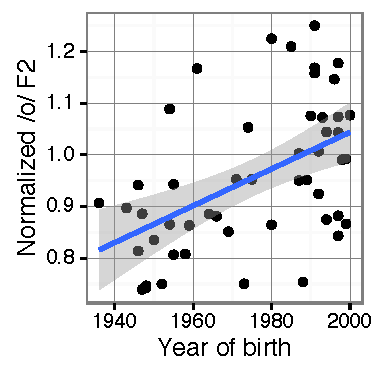
\includegraphics[scale=0.7]{ow_yob_small.pdf}}
\subfigure[]{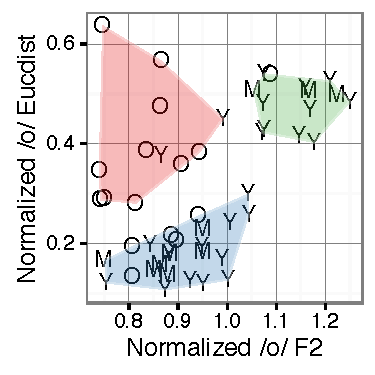
\includegraphics[scale=0.7]{ow_front_dip_small.pdf}}
%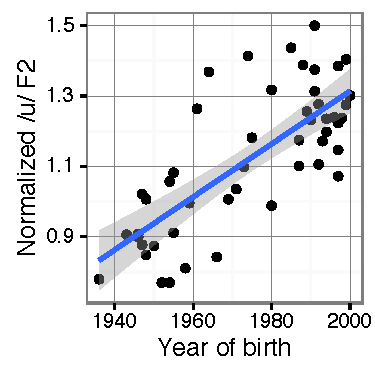
\includegraphics[scale=0.7]{uw_yob_small.pdf}
%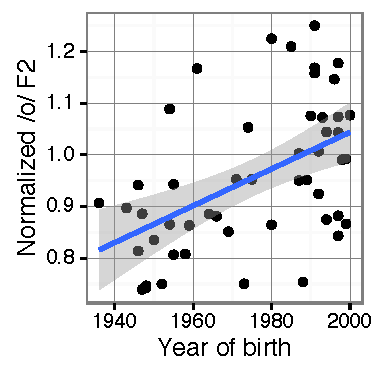
\includegraphics[scale=0.7]{ow_yob_small.pdf}
\end{figure}

Figure 1(c) plots mean Euclidean distance and F2 values for \textipa{/o/} in two-dimensional space, demonstrating how the fronting and diphthongization of this vowel interact. Letters represent three age categories (\textit{\textbf{Y}ounger / \textbf{M}iddle / \textbf{O}lder}) in 20-year bins. The shaded hulls show the output of density-based clustering (Ester et al., 1996), which identifies three groups of speakers -- those with back \textipa{/o/} realizations and middle/high Euclidean distances (primarily older speakers); those with back \textipa{/o/} realizations and low Euclidean distances, and those with fronted \textipa{/o/} realizations and high Euclidean distances (who are primarily younger speakers). Importantly, fronting occurs among speakers with diphthongal \textipa{/o/}, but speakers with monophthongal \textipa{/o/} appear to resist fronting, consistent with Haddican et al.'s (2013) findings.

In summary, the production data provide evidence for the fronting of \textipa{/u/} and \textipa{/o/}, consistent with previous work on this community (Haddican et al., 2013), and supporting the general observation that the co-fronting of \textipa{/u/} and \textipa{/o/} is common across varieties of English (Baranowski, 2008; Hall-Lew, 2009; Mesthrie, 2010). While \textipa{/u/} fronting appears to proceed in a relatively uniform manner, \textipa{/o/} fronting appears to be occurring more slowly and is spreading across the population in a less regular manner. The fronting of \textipa{/o/} appears to be restricted to diphthongal speakers -- while the fronting of monophthongal \textipa{/o/} is in principle possible, and attested in other Northern British varieties of English (Watt \& Tillotson, 2001), there appears to be an absence of fronted, monophthongal speakers in this sample. The patterning of these changes raises two questions:

\begin{enumerate}[i)]
\item{What causes \textipa{/u/} to front so rapidly and uniformly in comparison to \textipa{/o/}?}
\item{Why do younger speakers avoid fronted \textipa{/o/} monophthongs and back \textipa{/o/} diphthongs?}
\end{enumerate}
%A schematization of the trajectory of change in \textipa{/u/} and \textipa{/o/} is provided below. The oldest speakers in the sample produce relatively back \textipa{/u/} and \textipa{/o/} variants, and exhibit variation in terms of \textipa{/o/} diphthongization (i). The apparent conditional relationship between \textipa{/u/} and \textipa{/o/} fronting implies that change in \textipa{/u/} actuated before that in \textipa{/o/}, allowing an intermediate state to be posited (ii). At this stage, the centralization of \textipa{/u/} had begun, but \textipa{/o/} remained relatively back. The present stage of the change (iii) involves further fronting of \textipa{/u/}, and the sharp separation of speakers into two groups with regard to their \textipa{/o/} production -- those with very front diphthongs, and those with comparatively back monophthongs. 


%\begin{table}[ht]
%\centering
%\setlength{\tabcolsep}{0.5cm}
%\label{haddican-results}
%\begin{tabular}{llllllllll}
%&i.&ii.&iii.&\\
%\textipa{/o/} &    o $\sim$ \textipa{oU} &  o $\sim$ \textipa{oU}        &  o       &  \textipa{\textschwa y}                                  && \\
%\textipa{/u/} &  \textipa{u} &  \textipa{0} &  \textipa{y} & \textipa{y}                    &           &                  &\\
%&   &   &  &                    &           &                  &\\
%\end{tabular}
%\end{table}
Observing similar patterns in their data, Haddican et al. (2013) provide an explanation focusing on the local social indexicality of the changing vowels, consistent with the pattern of argument discussed in the introduction of this paper.  With regard to the relative uniformity of change in \textipa{/u/} vis-a-vis \textipa{/o/}, the authors propose that variation in \textipa{/o/} is strongly associated with socioeconomic status and `local' regional identity among York speakers, while the fronting of \textipa{/u/} is less important as a social-indexical resource. This relative lack of social indexing allows \textipa{/u/} fronting to propagate rapidly and relatively uniformly across the community. Such claims are reasonable, since the diphthongization of the mid vowels is known to be a shibboleth of Northern/Southern English identity, at least in production (Beal, 2004). 

The authors' second claim is that fronted, monophthongal \textipa{/o/} is associated with a stigmatized working-class stereotype, the `chav'. This stereotype, of a young person who is typically unemployed and engages in antisocial behaviour, has become a key feature of popular discourses around social class in the United Kingdom (see e.g. Hayward \& Yar, 2006). Haddican et al. (2013) provide convincing ethnographic evidence that this social category is important to younger York residents, and propose that the absence of fronted, monophthongal \textipa{/o/} in their younger informants' data may be explained by the enregisterment of this feature as part of `chav' speech.

 While Haddican et al.`s (2013) explanation is very reasonable based on their ethnographic data, it is formed primarily on the basis of production patterns, and warrants controlled testing. This raises the issue at the heart of the present work -- how can a set of claims regarding the role of social-indexical meaning in a sound change be evaluated? One way of thinking about such claims is to express them as a set of distributions over multidimensional phonetic space (Figure 2). These social categories may include macro-level meanings such as \textsc{local} or \textsc{working class}, or more locally-specific personae such as \textsc{chav}. Figure 2 includes an addition to the argument presented in Haddican et al. (2013); since back \textipa{/o/} diphthongs as well as fronted \textipa{/o/} monophthongs are absent from the speech of younger speakers in the present sample, it is reasonable to predict that both forms might be associated with the \textsc{chav} category.

\begin{figure}[ht]
\centering
\caption{Hypothesized mappings of indexical meanings to F2-Euclidean distance space}
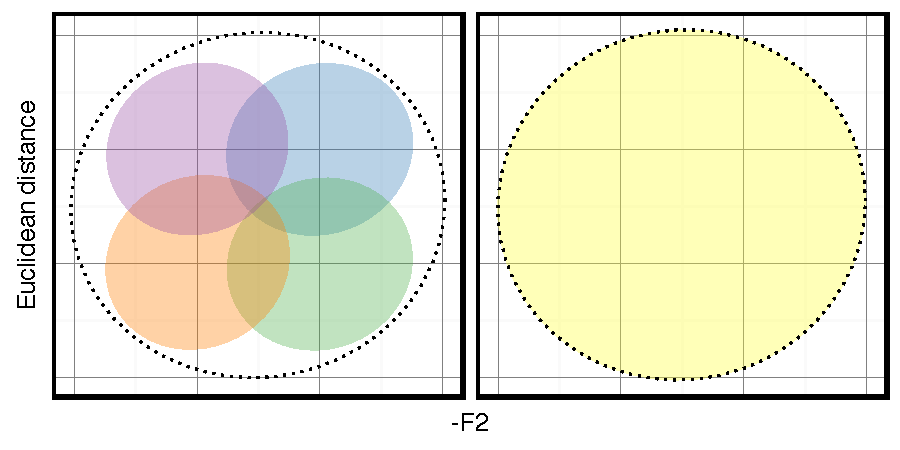
\includegraphics[scale=0.5]{predictions.pdf}
\end{figure}

The model in Figure 2 allows quantitative predictions to be formed regarding the social perception of the linguistic variables under study. For example, when a listener hears a talker use a back, diphthongal variant of \textipa{/o/}, it might be expected that they would assign that talker to the \textsc{chav} category. With increasing fronting, that listener would be increasingly more likely to assign \textsc{middle class} to that talker. This pattern of reasoning can be extended across all combinations of phonetic parameters and social categories (see section 3.4). The following section will describe a social perception experiment which aimed to test the predictions of the model in Figure 2, quantifying the extent to which York listeners associate the proposed social categories with \textipa{/u/} and \textipa{/o/} variation. 

\section{The social perception of \textipa{\textipa{/u/}} and \textipa{\textipa{/o/}} variation}

\subsection{Auditory stimuli}

Auditory stimuli consisted of resynthesized tokens of the words \textit{too}, \textit{food} (\textipa{/u/}), \textit{toast} and \textit{so} (\textipa{/o/}), read by a 24-year-old middle-class speaker from York. The \textipa{/u/} stimuli included examples of three levels of fronting, as well as three identical tokens with lowered onsets, resulting in more diphthongal tokens (3a). The \textipa{\textipa{/o/}} stimuli included tokens representing three steps of fronting of monophthongal variants and three steps of two types of fronting (targeting the vowel onset and offglide) across diphthongal tokens. These included a back diphthongal realization, two steps of fronting at the vowel onset, and two steps of fronting of the offglide (3b). 

\begin{figure}[ht]
\caption{\textipa{/u/} and \textipa{/o/} variants used in the perception experiment}
\centering
\vspace*{-.5cm}
\subfigure{
\centering
\scriptsize
\begin{tabular}{llllll}
&\normalsize{(a)}&&&&\\
                  &           & \textit{Fronting}          &             &                   &\\
            &  \multicolumn{3}{l}{$\xleftarrow{\hspace*{3cm}}$  }  &                           \vspace*{-0.1cm}   \\ 
     \multirow{5}{*}{$\rotatebox[origin=c]{90}{$\underleftarrow{\mathsf{\textit{Diphthongization}}}$}$}        
                      
 &&&&       &\\
        &\LARGE{\textbf{\textipa{Yu}}}&\LARGE{\textbf{\textipa{0u}}}&\LARGE{\textbf{\textipa{Uu}}}&&\\
                       &&&&&\\

               & \LARGE{\textbf{\textipa{eu}}}&\LARGE{\textbf{\textipa{9u}}}&\LARGE{\textbf{\textipa{7u}}}&&\\
\end{tabular}} 
\hspace*{-1cm}
\subfigure{
\scriptsize

\begin{tabular}{llllll}
\vspace*{0.2cm}\\
&\normalsize{(b)}&&&&\\
                  &           & \textit{Fronting}          &             &                   &\\ \vspace*{-0.1cm}
                &  \multicolumn{3}{l}{$\xleftarrow{\hspace*{3cm}}$  }   &                              \\
\multirow{5}{*}{$\rotatebox[origin=c]{90}{$\underleftarrow{Diphthongization}$}$}                 &&&& &                \\
               & \LARGE{\textbf{\textipa{\o:}}}&\LARGE{\textbf{\textipa{8:}}}&\LARGE{\textbf{\textipa{o:}}}&&\\
               &&&&&\\
        &\LARGE{\textbf{\textipa{eU}}}&\LARGE{\textbf{\textipa{9U}}}&\LARGE{\textbf{\textipa{oU}}}&&\\
                     &&&&&\vspace*{-0.2cm}\\ 
                   &\LARGE{\textbf{\textipa{9y}}}&\LARGE{\textbf{\textipa{90}}}&&&\\
\end{tabular}}
\end{figure}

\subsection{Visual stimuli}

Visual stimuli consisted of eight images representing individuals of different ages (older vs younger), different occupations (working class vs middle class) and of different regional background (urban vs rural).  The social dimensions of older/younger, working-class/middle-class, and urban/rural were included based on the findings of a set of ethnographic interviews conducted prior to the main data collection phase, as well as the claims made by Haddican et al. (2013). Evidence from the ethnographic interviews suggests the categories \textsc{urban} and \textsc{rural} are central to York speakers' construal of a `local' Yorkshire identity; in light of this, the present analyses treat selections on the urban/rural dimension as a proxy for Haddican et al.`s `localness'. Each stimulus image contained three components -- an image of a face (providing information about the character's age), an image of a place of work/study (providing information about the character's social status) and an image of an urban or rural location (providing information about the regional background of the character). The eight images represent all possible combinations of these three social dimensions, shown in Figure 3.7.

\begin{figure}[ht]
\caption{Visual stimuli}
\centering
\begin{tabular}{ccccc}
\multirow{2}{*}{$\rotatebox[origin=t]{90}{$\overbrace{\rule{0.5cm}{0pt}\mathsf{\textit{Rural}}\rule{0.5cm}{0pt}}$\hspace*{-2cm}}$} &
\includegraphics[scale=0.25]{M_O_MC_L_1.png} & 
\includegraphics[scale=0.25]{M_Y_MC_L_1.png} 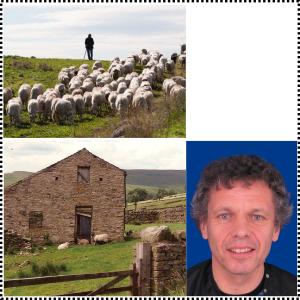
\includegraphics[scale=0.25]{M_O_WC_L_1.png} &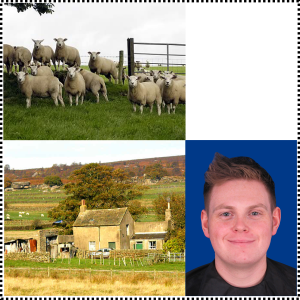
\includegraphics[scale=0.25]{M_Y_WC_L_1.png} \\ 
 $\rotatebox[origin=t]{90}{\hspace*{1.5cm}$\overbrace{\rule{0.5cm}{0pt}\mathsf{\textit{Urban}}\rule{0.5cm}{0pt}}$}$
    &
\includegraphics[scale=0.25]{M_O_MC_NL_1.png} & 
\includegraphics[scale=0.25]{M_Y_MC_NL_1.png} 
\includegraphics[scale=0.25]{M_O_WC_NL_1.png} & 
\includegraphics[scale=0.25]{M_Y_WC_NL_1.png}\\
\end{tabular}
\vspace*{-1.5cm}
\end{figure}
\begin{figure}[!htpb]
\centering
\begin{tabular}{lllll}


    &\multicolumn{4}{l}{
    $\underbrace{\rule{1cm}{0pt}{\textit{Age: Older/Younger}}\rule{1cm}{0pt}}$$\underbrace{\rule{1cm}{0pt}{\textit{Age: Older/Younger}}\rule{1cm}{0pt}}$}\\

    &\multicolumn{4}{l}{
$\underbrace{\rule{2.5cm}{0pt}{\textit{Social class: Middle/Working}}\rule{2.5cm}{0pt}}$}\\
   \end{tabular}
\end{figure}

The characters were designed to be feasible York personae based on the ethnographic interview data. For example, the intersection of older, middle-class, and rural is represented by a doctor in a rural Yorkshire village (top, left-hand cell of Figure 4), while the corresponding middle-class character is represented as a middle-aged businessman associated with a well-known insurance company (bottom, left-hand cell of Figure 4). In all cases, the choice of component images reflects comments made by participants during the ethnographic interviews. A key claim made by Haddican et. al. (2013) is that fronted monophthongal \textipa{/o/} variants are associated the `chav' stereotype. In this experiment, the `chav' is treated as the intersection of the urban, young and working-class dimensions, represented by the character in the bottom, right-hand cell of Figure 4.

\subsection{Experimental task}

Participants were told that they were listening to an actor preparing for a role in a sitcom set in York. In the training phase of the experiment, they were asked to categorize the visual stimuli based on a series of prompts (e.g. `Which character is older', `Which character is working-class?'). They achieved this with an accuracy of 96\%. During the main experiment, participants saw two images per trial, heard a speech token, and were asked to select the character which they thought the actor was pretending to be. The two images on each trial differed in terms of one of the three social dimensions, with the remaining two kept constant between each image pair.


\subsection{Predictions based on Haddican et al. (2013)}

The key claims of Haddican et al (2013) are that \textipa{/o/} diphthongization is associated with social class and local regional identity; that \textipa{/o/} fronting is relatively socially unmarked; and that fronted, monophthongal \textipa{/o/} is associated with the `chav' stereotype, particularly among younger speakers. In section 2 it was argued that this second proposal can be extended to include back, diphthongal \textipa{/o/}, given the evidence of younger speakers' avoidance of these forms. In order to bring the perception data to bear on these claims, they can be framed as statements regarding the probability of a selection on each social dimension, which are summarized below. 
\begin{enumerate}[(a)]
\item{The probability of a \textsc{working-class} selection should be higher for monophthongal \textipa{/o/} variants than diphthongal \textipa{/o/} variants.}
\item{The probability of a \textsc{rural} selection should be higher for monophthongal \textipa{/o/} variants than diphthongal \textipa{/o/} variants.}
\item{Variation in \textipa{/u/} should have a no effect on the probability of a \textsc{working-class} or \textsc{rural} selection, or will have a smaller effect than variation in \textipa{/o/}.}
\item{The probability of a \textsc{chav} selection should be higher for fronted, monophthongal \textipa{/o/} than back, monophthongal \textipa{/o/}.}
\item{The probability of a \textsc{chav} selection should be higher for back, diphthongal \textipa{/o/} than fronted, diphthongal \textipa{/o/}.}
\item{(d) and (e) will interact with listener year of birth, with the largest effects among younger listeners.}
\end{enumerate}

\subsection{Model selection}

These probabilities were estimated using multilevel logistic regression models fit for each vowel on each social dimension. Separate models were fit for the \textsc{working class} dimension (all \textsc{working class} vs all \textsc{middle class} images), the \textsc{rural} dimension (all \textsc{rural} vs all \textsc{non-rural} images), and the \textsc{chav} category (the \textsc{chav} image vs all others).  Baseline models predicted the selection of the social category modeled with random intercepts, by-listener random slopes for \textit{Variant}, and random slopes for sound sample within \textit{Variant}. The relative fit of these models was compared with more complex ones by minimizing the AIC criterion. Models tested included terms for the variant heard, the listener's year of birth, and the interactions of those factors (Table 1). Additionally, three indices derived from a social identity questionnaire were included: a socioeconomic status index (reflecting traditional measures of SES), a local identity index (reflecting e.g. the extent to which listeners are involved in local heritage events; whether or not they plan to stay long term in York), and a mobility index (reflecting e.g. the extent to which the are in contact with people from outside of York, and the extent to which they travel).  Significance tests were conducted for each model term using likelihood-ratio tests (Table 2).
 

 \begin{table}[ht]
 \small
 \caption{Formulae for best-fitting models of social selections}
\centering
\begin{tabular}{lll}
  \hline
 &\textipa{/o/}&\textipa{/u/} \\ 
   \hline

 \textbf{\textsc{working class}}&$\sim$ \textit{Variant * Mobility + random terms}&$\sim$ \textit{Variant * Age + random terms}\\ 
\textbf{\textsc{rural}}&$\sim$ \textit{Variant + random terms}&$\sim$ \textit{random terms}\\ 
\textbf{\textsc{chav}}&$\sim$ \textit{Variant * Age + random terms}&$\sim$ \textit{Variant * Age + random terms}\\ 
\end{tabular}
\end{table}


 \begin{table}[ht]
 \small
 \caption{Likelihood ratio tests for significance of model terms}
\centering
\begin{tabular}{llllllll}
  \hline
 \textipa{/o/}& Chisq & Df & P(Chisq) & \textipa{/u/}&Chisq & Df & P(Chisq) \\ 
  \hline
 \textbf{\textsc{working}}&&&  &\textbf{\textsc{working}}&&&\\ 
  \textbf{\textsc{class}}&&&  & \textbf{\textsc{class}}&&&\\
  \textit{Variant}& 51.64 & 7.00 & $<$0.0001 &  \textit{Variant}& 27.29 & 5.00 & $<$0.0001 \\  
  \textit{Variant*Mobility}& 18.42 & 8.00 & 0.02 &  \textit{Variant*Age}& 16.18 & 6.00 & 0.01 \\ 
\textbf{\textsc{rural}}&&&  & \textbf{\textsc{chav}}&&&\\ 
  \textit{Variant}& 17.37 & 7.00 & 0.01 &  \textit{Variant}& 27.74 & 5.00 & $<$0.0001 \\ 
\textbf{\textsc{chav}}&&& &  \textit{Variant*Age}& 19.25 & 6.00 & $<$0.01 \\ 
  \textit{Variant}& 49.39 & 7.00 & $<$0.0001&&&& \\ 
  \textit{Variant*Age}& 19.68 & 8.00 & 0.01&&&& \\
   \hline
\end{tabular}
\end{table}


In terms of \textsc{working class} and \textsc{chav} selections, the models for both \textipa{/u/} and \textipa{/o/} include the \textit{Variant} term, confirming that listeners were able to use variation in these vowels as a cue to socioeconomic status and to the `chav' subcategory. \textsc{rural} selections were reliably affected by variation in \textipa{/o/}, but not \textipa{/u/}. The best models for \textsc{working class} also include interaction terms for listener mobility (\textipa{/o/}) and year of birth (\textipa{/u/}), and the best models for \textsc{chav} include interaction terms for year of birth, indicating that listeners of different ages and social backgrounds behaved differently in the social perception task. At first glance, some of these results are surprising -- given the relatively uniform adoption of \textipa{/u/} fronting evident in the production data, it was predicted that \textipa{/u/} variation would be relatively socially unmarked in perception. However, the fact that \textipa{/u/} variants had a significant effect on listeners social selections suggests otherwise.


\subsection{Results: Main effects}
\subsubsection{\textipa{/u/}}
\begin{figure}[ht]
\centering
\caption{Main effects for \textipa{/u/}}
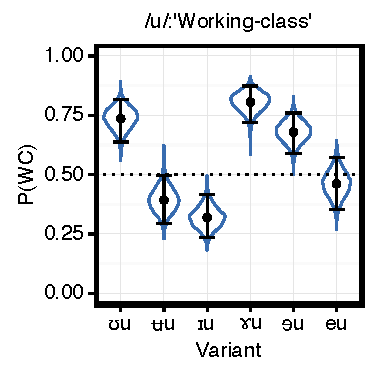
\includegraphics[scale=0.65]{uw_class.pdf}
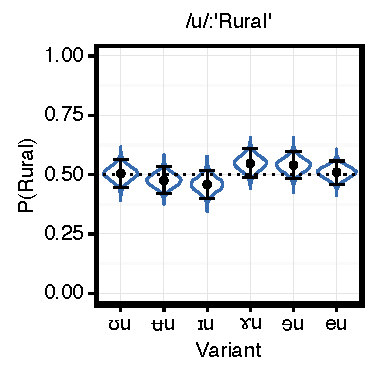
\includegraphics[scale=0.65]{uw_local.pdf}
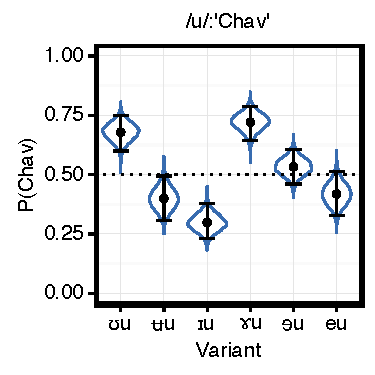
\includegraphics[scale=0.65]{uw_chav.pdf}
\end{figure}
Figure 5 demonstrates how listeners' social selections were affected by variation in \textipa{/u/}. The points represent the population-level estimates of the probability of each selection, with confidence intervals estimated through 10000 posterior samples. Despite predictions to the contrary, there is a clear effect of fronting on \textsc{working-class} selections, whereby fronter \textipa{/u/} variants are more likely to cue middle-class selections and back variants are more likely to cue working-class selections. \textipa{/u/} diphthongization seems to be weakly associated with \textsc{working class}, in that diphthongization weakens the effect of fronting, evident in the shallower slope of fronting across more diphthongal \textipa{/u/} variant. A similar pattern is visible in the \textsc{chav} selections; again in spite of the prediction that \textipa{/u/} variation would not affect selections of this category. The results for \textsc{rural} selections are more consistent the predictions made previously -- while \textipa{/u/} diphthongs were marginally more likely to cue a \textsc{rural} selection, fronting appears to have had little effect on listeners' selections; recall that \textit{Variant} was not included in the best-fitting model. Overall, the results for \textipa{/u/} contrast strongly with the predictions formed earlier, where it was suggested that \textipa{/u/} variation would be perceived as relatively socially unmarked (at least with regard to socioeconomic status/regional identity), given its lack of social stratification in production and comparatively rapid incrementation. This is a somewhat suprising result -- while cases where variants stratify socially in production without attracting social indexing are widely often reported (e.g. Labov's (1972) `markers'), here there seems to be evidence of a consistent perceptual evaluation in the absence of stratification in production. 

\subsubsection{\textipa{/o/}}
\begin{figure}[ht]
\centering
\caption{Main effects for \textipa{/o/}}
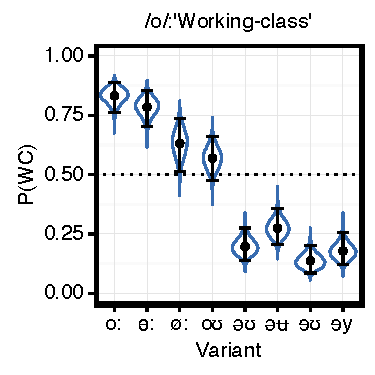
\includegraphics[scale=0.65]{ow_class.pdf}
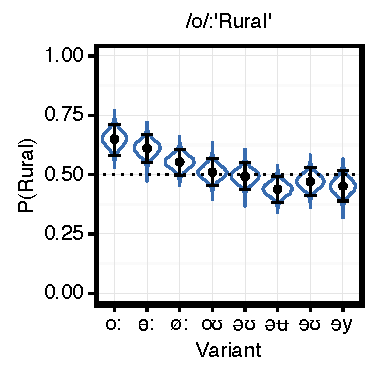
\includegraphics[scale=0.65]{ow_local.pdf}
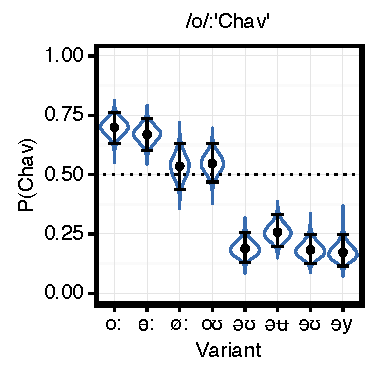
\includegraphics[scale=0.65]{ow_chav.pdf}
\end{figure}

Figure 6 visualizes the effect of the auditory stimuli on social selections for \textipa{/o/}. As predicted in section 3.4, there is a clear effect of diphthongization on \textsc{working class} selections, with more diphthongal variants reliably cueing the selection of a middle-class image, and monophthongal variants cueing the selection of working-class image. The only exception to this pattern is back, diphthongal \textipa{/o/}; since the confidence interval for this variant crosses zero, it cannot be concluded that this variant had a reliable effect in either direction. However, the fact that the interval is biased above the p=.5 line suggests that at least some listeners tended to select working-class images when hearing a back diphthong. This suggests that the front-back dimension of \textipa{/o/} had an unexpected effect on listeners' selections, with back variants heard as more \textsc{working class} than fronted variants. Monophthongs all reliably predict the selection of a working-class image, but the strength of this effect weakens for more fronted variants. Note that the tendency for fronting to shift perceptions away from \textsc{working class} holds for both diphthongs and monophthongs, and is the exact opposite to what was predicted based on the production data. In terms of \textsc{rural} selections, \textipa{/o/} shows a weak but reliable effect for monophthongal variants, which is broadly consistent with our earlier predictions -- listeners reliably map \textipa{/o/} monophthongs to the \textsc{rural} category, although this is weakly mediated by fronting in a similar manner to the \textsc{working class} selections. Turning to \textsc{chav} selections, a key prediction based on Haddican et al.'s (2013) proposal was that fronted \textipa{/o/} monophthongs would be associated with this category. However, the data for \textipa{/o/} provide no support for this proposal; if anything, they suggest the opposite. While the most back \textipa{/o/} variants reliably cue \textsc{chav} selections, fronted \textipa{/o/} shows no reliable effect, and the overall trend is for fronting to \textit{lower} the probablity of a \textsc{chav} selection -- again, the opposite to what was predicted.


\subsection{Results: Listener variation}
A further prediction made in section 3.4 was that listeners would vary in their social perception of variation in \textipa{/o/} and \textipa{/u/}. In particular, it was predicted that the association of fronted \textipa{/o/} monophthongs and back \textipa{/o/} diphthongs with the \textsc{chav} category would be strongest among younger listeners. While there was no evidence of such an association, let alone the predicted interaction, there is convincing evidence that listeners varied in their perceptual behaviour in interesting ways. Certain groups of individuals (younger, more mobile listeners) appear to be more perceptually sensitive to variation in the vowels under study, in the sense that they map variation in \textipa{/o/} and \textipa{/u/} more consistently to the social categories tested. There is also evidence of a change in the variants which are enregistered as part of `chav' speech, demonstrated in age-stratified variation in the experimental data. These effects are discussed below.
\subsubsection{\textsc{working class} selections}
\begin{figure}[ht]
\centering
\caption{Interaction effects: \textsc{working class} selections}
\subfigure[]{
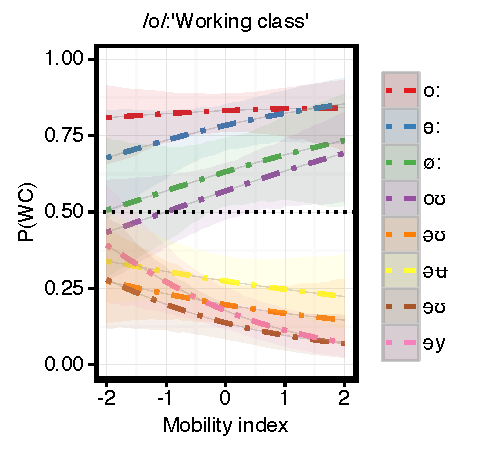
\includegraphics[scale=0.6]{ow_class_dim3.pdf}
}
\subfigure[]{
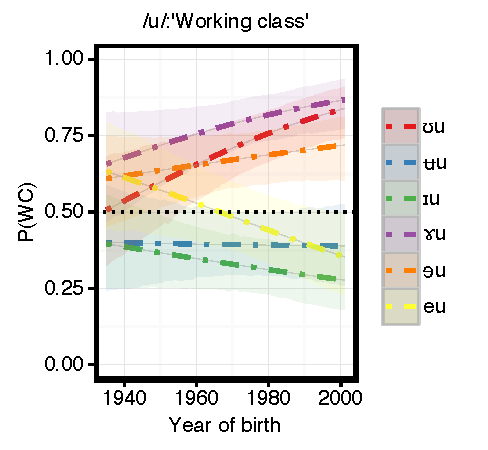
\includegraphics[scale=0.6]{uw_class_age.pdf}
}
\end{figure}
Figure 8 demonstrates variation in social class selections as a function of listener year of birth and the mobility index. For \textipa{/o/}, there is a significant effect of listener mobility (8a), with more mobile listeners generally more sensitive to the monophthong-diphthong distinction as a cue to socioeconomic status. The largest variation appears to be in the perception of the most fronted diphthong and most back monophthong -- these variants have a limited effect on the responses of less mobile listeners, suggesting that those listeners hear them as comparatively unmarked. In contrast, more mobile listeners tend to associate these variants with middle-class characters. \textipa{/u/} selections show no evidence of variation in terms of mobility, but a significant effect of listener age (8b). Older listeners are generally less sensitive to fronting as a cue to socioeconomic status. Neither of these effects were predicted by Haddican et al.`s (2013) account of the social indexicality of \textipa{/u/} and \textipa{/o/}, but they still warrant explanation. In the case of \textipa{/o/}, it may be that more mobile individuals' experience with external varieties makes them better able to notice diphthongization and interpret it as an indexical cue -- this would be consistent with the findings of Jefferies (2015), whose results suggest a crucial role of social network structure in the acquisition of sociolinguistic competence. It is less clear why younger listeners would be more sensitive to \textipa{/u/} fronting as a cue to social class, particularly given the lack of evidence that fronted \textipa{/u/} indexes class in production. One suggestion might be that this pattern represents the incipient attachment of social meaning to \textipa{/u/} variation -- younger speakers have detected (stylistic, regional, or age-related) variation in \textipa{/u/}, and have begun to map that variation on to class-related social meanings. This results in some speakers hearing fronting as a `middle class' feature, even though middle-class speakers in their community do not actually produce this feature distinctly from other groups. If this is the case, it would not be surprising if fronted \textipa{/u/} was to emerge as a productive index of socioeconomic status in future generations, as the indexical mappings of today's younger speakers become part of the community norms.

\subsubsection{\textsc{chav} selections}
\begin{figure}[ht]
\centering
\caption{Interaction effects: \textsc{chav} selections}
\subfigure[]{
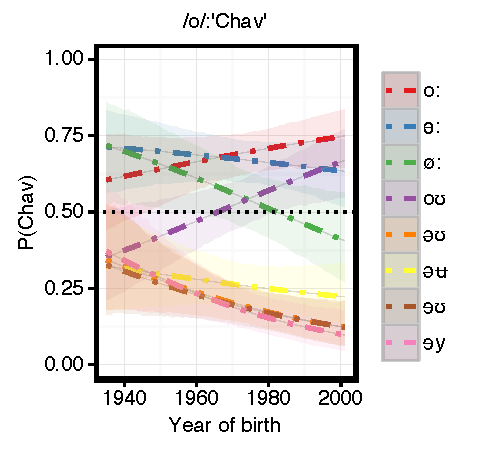
\includegraphics[scale=0.6]{ow_chav_age.pdf}}
\subfigure[]{
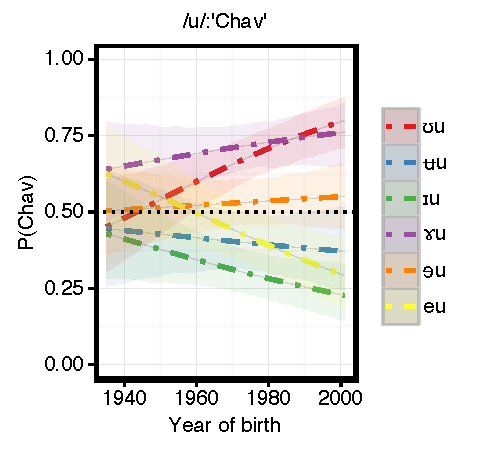
\includegraphics[scale=0.6]{uw_chav_age.pdf}}
\end{figure}
Figure 8 demonstrates the interaction of listener year of birth and variant heard on \textsc{chav} selections. For \textipa{/u/} (8b), the effect of age is similar to that for \textsc{working-class} selections -- younger listeners map the back-front dimension of \textipa{/u/} more reliably to the \textsc{chav} character than older listeners, perhaps representing the early stages of the enregisterment of \textipa{/u/} as part of `chav' speech. The most interesting effect in the \textipa{/o/} data is the `cross-over' pattern involving the interaction of fronting and diphthongization. Where \textipa{[8:]} reliably cues a \textsc{chav} selection among older listeners, younger listeners seem to slightly favor a \textsc{non-chav} selection when hearing this variant; conversely, \textipa{[oU]} disfavours a \textsc{chav} selection among older listeners, but reliably maps to \textsc{chav} among younger listeners. While it may be inappropriate to interpret social perception data using an apparent-time construct, one interpretation of this pattern is that the phonetic cues associated `chav' speech are undergoing change -- where the combination of fronting and monophthongization in \textipa{/o/} was historically heard as `chav' (or linked to a similar social category), this association may have weakened over time, replaced by the combination of backness and diphthongization. However this listener-level variation is understood, it is clear that the social-indexical interpretation of phonetic variation may differ across subgroups of a single speech community, consistent with recent findings regarding group-level variation in sociolinguistic perception (Walker et al., 2014).

\section{Conclusion}
This paper has demonstrated how a typical pattern of argument in sociolinguistics -- inferring the social significance of pronunciation variants from production data -- can lead to conclusions which contrast strongly with the results of controlled elicitation methods. Although the hypothesised association between \textipa{/o/} diphthongization and socioeconomic status was well-supported by the perceptual data, the remaining predictions lacked empirical support, and were in some cases directly contradicted by the results of the experiment. While the relative uniformity of \textipa{/u/} fronting in York was interpreted as reflecting a lack of local social indexing by Haddican et al. (2013), \textipa{/u/} fronting was shown to be a reliable cue to socioeconomic status in the perception data. Furthermore, building on Haddican et al.`s (2013) account of variation and change in this community, it was predicted that fronted, monophthongal and back, diphthongal \textipa{/o/} would be strongly associated with working class status and the `chav' stereotype. However, the experimental results run in the opposite direction  -- fronted \textipa{/o/} monophthongs were \textit{less} likely to cue a \textsc{chav} selection than back monophthongs. Taken together, these results show that even a very reasonable, ethnographically-informed argument regarding indexical meaning can fail to find support once testable predictions regarding listener behaviour are formed and evaluated. This highlights the value of triangulating sources of data when reasoning about the factors contributing to the outcome of a sound change.

One surprising finding of the present work was that some listeners consistently mapped fronted \textipa{/u/} variants to middle-class images, despite the lack of evidence for the social stratification of this form in production. Methodologically, this demonstrates that drawing on multiple sources of evidence when studying social indexicality may not only be helpful in avoiding positing a social meaning where none exists, but may also help us detect indexical associations which are not yet observable in production behaviour. From a theoretical perspective, this finding is interesting in that it is commonly assumed that social stratification in production occurs \textit{before} listeners attach social evaluations to variation -- this is implicit, for example, in Labov's (1972) indicator-marker-stereotype hierarchy, as well as in more recent discussions of sociolinguistic salience (e.g. R\'acz, 2013). However, it seems that, under certain circumstances, listeners can hear forms as `middle class' without those forms indexing socioeconomic status in production. As suprising as this result may be, it resonates with the recent findings of Barron-Lutzross (2015) regarding the perception of lesbian speech styles. Listeners were shown to consistently rate female talkers with higher average F2 as more feminine and less likely to be a lesbian, despite there being no evidence for the corresponding relationship in production. These results suggest that the assumed implicational relationship between the patterning of variants in production and social evaluation may not describe the full range of possiblities by which social meaning may be associated with language variation.

A further important finding of the present work is that listener groups vary in the way they map phonetic variation on to social categories. In York, it seems that younger, more mobile listeners (that is, speakers who are more geographically mobile and have weaker ties to the local community), attend more to \textipa{/o/} diphthongization and \textipa{/u/} fronting as a cue to socioeconomic status than less mobile speakers. Additionally, there is evidence that younger speakers differ from older speakers in which forms they map to the \textsc{chav} category. One question which remains to be resolved is the degree to which this variability in social perception reflects differences in the indexical meanings relevant to different social groups, or more general differences in listeners' ability to notice and respond to sociophonetic cues. This second possibility has important implications for ongoing work on the role of individual differences in the actuation and spread of sound changes (e.g. Yu, 2015). Evidence that some listeners are generally more sensitive to indexical cues than others might provide part of the answer to the fundamental question of how linguistic innovations propagate. It may be that those listeners with a higher propensity to assign social significance to variability in the speech of others are also more likely to employ certain innovations in their own speech, contributing to the spread of those forms through the speech community.

\bibliographystyle{pwpl.bst}
\nocite{*}
\bibliography{reviewbib_short.bib}
\end{document}